
\subsection{Bewegungsgleichungen}
Im folgenden werden wir uns an die häufige Notation halten, Vektoren fett zu schreiben. Wir gehen außerdem davon aus, das man die Existenz und Größe einer unbekannten anomalen Beschleunigung überprüfen will.

Die Bewegung der Raumsonden wird durch Lösen der Bewegungsgleichungen bestimmt, welche sich am einfachsten wie folgt schreiben lassen:
\begin{equation}
\frac{d{\bf v}}{dt}={\bf a_N} + {\bf a_S} + {\bf a_P} + ...
\end{equation}
und
\begin{equation}
\frac{d{\bf r}}{dt}={\bf v}
\end{equation}
Dabei ist $\bf a_N$ die Beschleunigung durch die Gravitationskraft, $\bf a_S$ die Beschleunigung durch den solaren Strahlungsdruck und $\bf a_P$ die Pioneeranomalie. Weitere Effekte können durch zusätzliche Terme berücksichtigt werden; dies erhöht die Genauigkeit, ändert jedoch nichts an der Tatsache, dass die Anomalie existiert, deshalb ignorieren einige Arbeiten diese Terme. Wir werden einige dieser Effekte im Kapitel \ref{klassisch} kennen lernen.
%Hier auslisten was noch berücksichtigt werden kann?
Die gravitative Beschleunigung kann durch Newtonsche Anziehung der Massen berechnet werden:
\begin{equation}
{\bf a_N} = \sum_j \frac{GM_j\left({\bf r_j}-{\bf r}\right)}{\left| {\bf r_j}-{\bf r} \right|^3}
\end{equation}
Wobei hier $M_j$ die Massen, $\bf r_j$ die Positionen der Massen und $\bf r$ die Position der Sonde sind.
Für eine höhere Genauigkeit kann man relativistische Einflüsse auf die gravitative Beschleunigung berechnen. So verwenden Anderson et al. in ihrer Arbeit den parametrisierten Post-Newtonschen-Formalismus (PPN), einer Vereinfachung von Einsteins Gravitationsgleichung für schwache Felder und langsame Geschwindigkeiten.
Die Details dieses Formalismus gehen jedoch weit über diese Arbeit hinaus.
Die mit Abstand wichtigste Masse ist natürlich die der Sonne, aber auch die Planeten und der Mond müssen berücksichtigt werden.
Während Anderson\cite{Anderson2002} auch die größten Asteroiden (ca. 0,2 Erdmassen) und Kometen – wenn auch nur mit dem Newtonschen Gravitationsgesetz – berücksichtigte, ignorierte Markwardt diese völlig.
Grundsätzlich lassen sich die Himmelskörper als Punktmassen beschreiben, lediglich wenn sich die Sonde in der Nähe eines Planeten befindet, muss die Auswirkung der Ausdehnung und idealerweise auch der Einfluss der Monde der Planten genauer berechnet werden. Dies ist beim Vorbeiflug an Jupiter (Pioneer 10 und 11) und Saturn (Pioneer 11) der Fall.
Die Positionen und Massen der Planeten wurden in den früheren Analysen aus der Ephemeride
DE402, später aus DE405 durch Interpolation entnommen
\footnote{\textit{``Jet Propulsion Laboratory Development Ephemeris''} sind durch
numerische Integration erzeugte Ephemeriden welche primär für die Raumfahrt gedacht sind.}\cite{Anderson2002}.

Den Druck durch die von der Sonne ausgehende Strahlung $\bf a_S$ berechnet man durch:
\begin{equation}
a_S = \frac{\mathcal{K}f_\odot A_P}{c M_P} \left| \frac{1\ \mathrm{AU}}{{\bf r}-{\bf r_\odot}} \right|^2 \cos\theta
\end{equation}
Dabei ist $\bf r_\cdot$ die Position der Sonne im Koordinatensystem, $M_P$ ist die Masse der Sonde, $A_P$ die von der Sonnenstrahlung betroffene Sondenoberfläche, $f_\odot$ die Solarkonstante, $\mathcal{K}$ der Reflexionskoeffizient und $\theta$ der Winkel unter dem die Oberfläche von der Sonnenstrahlung getroffen wird.
Zur Vereinfachung wird für $A_P$ die Fläche der Antenne verwendet.
Da der Winkel $\theta$ immer unter 1.5° ist wird er zu $\theta = 0\degree$ vereinfacht, was lediglich zu einem Verlust an Genauigkeit von $< 4 \cdot 10^{-12} \frac{cm}{s^2}$ führt\cite{Markwardt2002}.

Die Pioneer-Anomalie – deren Überprüfung und Bestimmung das Ziel der Untersuchung ist – wird durch folgenden Term ausgedrückt:
\begin{equation}
a_P(t) = \left( a_P(0) + j_pt\right){\bf \hat{r}}
\end{equation}
Wir betrachten also einen konstanten Teil $a_P(0)$ und einen mit der Zeit ansteigenden Teil $j_p$. Der Richtungsvektor $\bf \hat{r}$ zeigt von der Sonde in Richtung Sonne (Zur genauen Richtung der Anomalie in Kapitel XXX mehr).

\begin{figure}[htbb]
\begin{minipage}[t]{.8\linewidth}
	\centering
	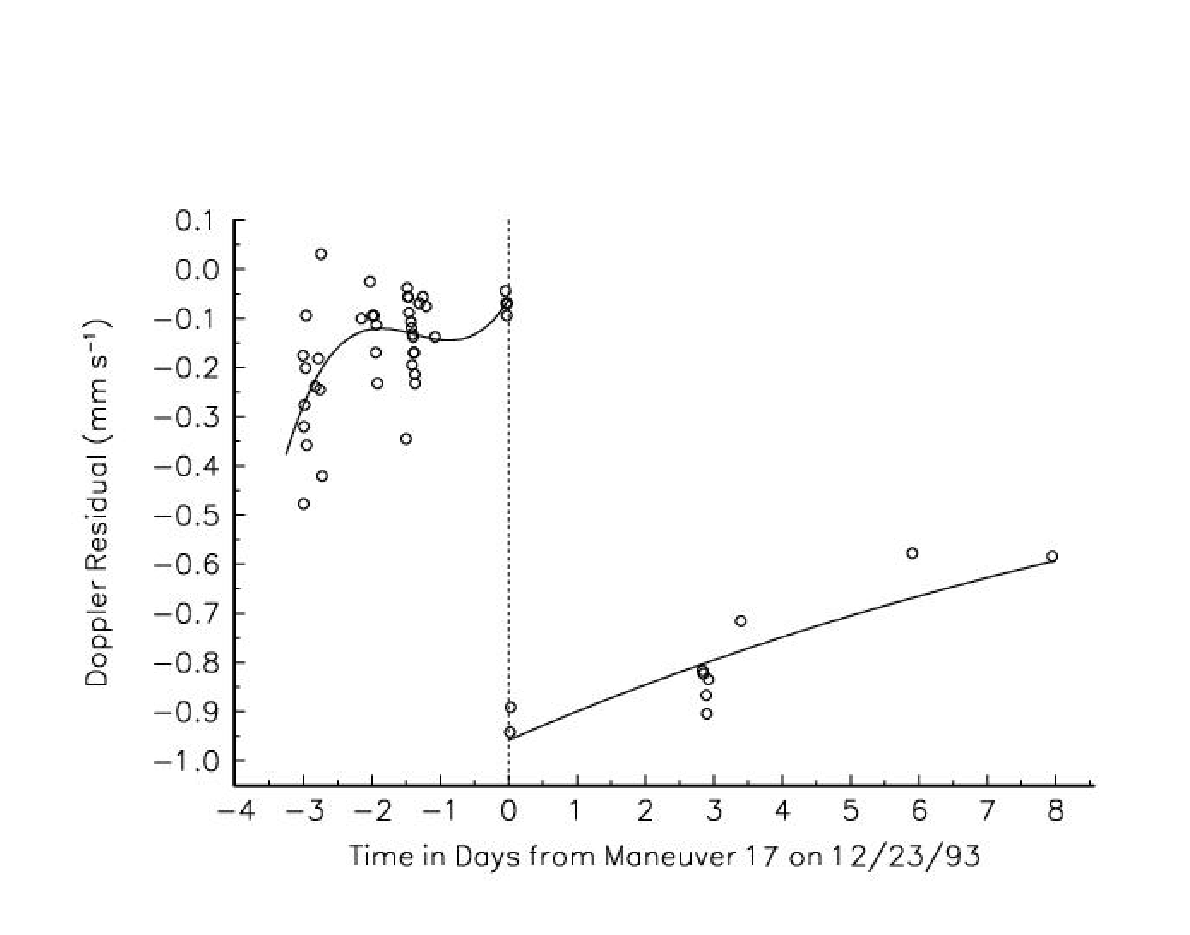
\includegraphics[width=\linewidth]{images/manoever}
  \caption{Doppler-Verschiebung durch ein Manöver (Nummer \#17, aus dem von Anderson\cite{Anderson2002} analysiertem Intervall; am 23. Dezember 1993)}\label{fig:manoever}
\end{minipage}
%\hfill
%\begin{minipage}[t]{.48\linewidth}
	\centering
%	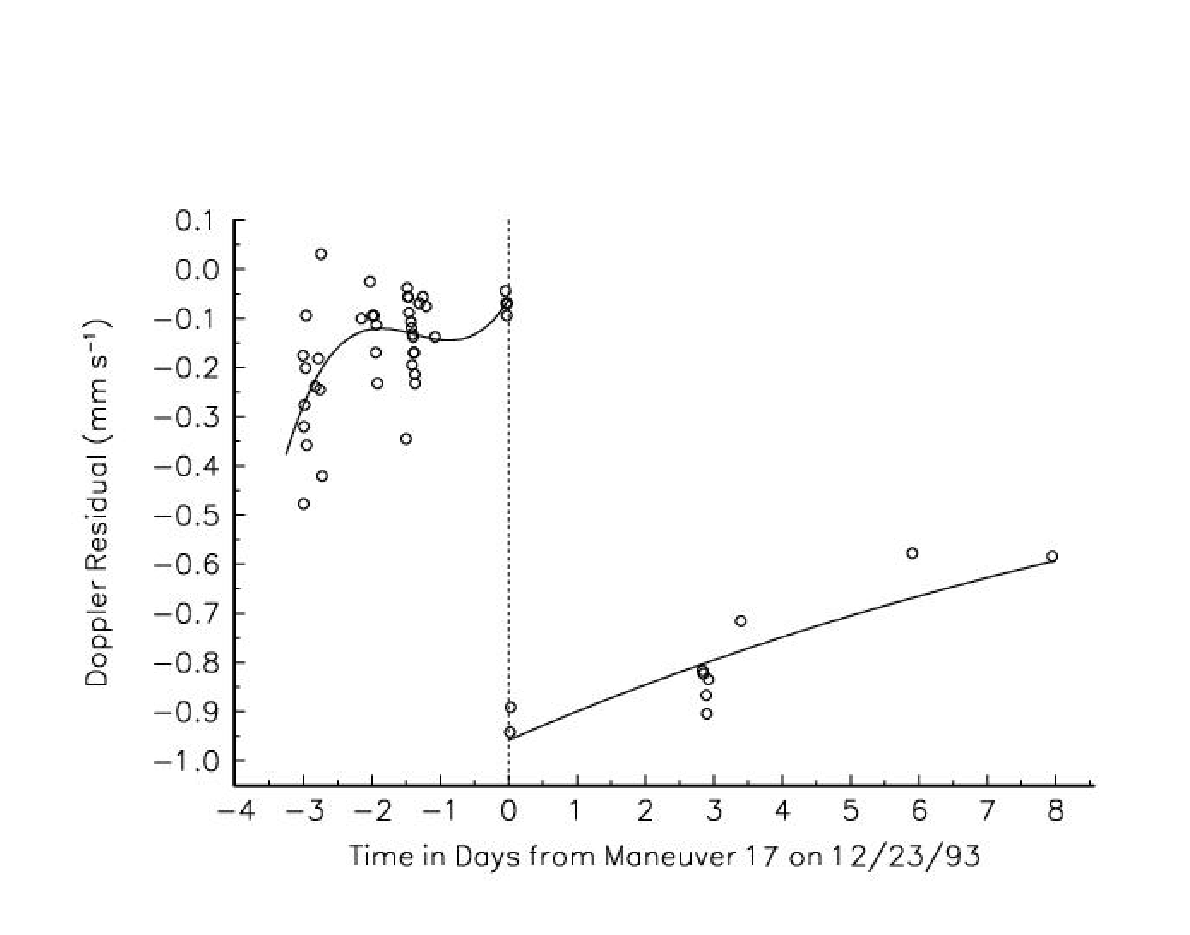
\includegraphics[width=\linewidth]{images/manoever}
%	\label{fig:manoever}
%  \caption{ }
%\end{minipage}
 \end{figure}

% Wohin mit den Manövern?
Außerdem muss man die zahlreichen kleinen Manöver berücksichtigen. Diese waren notwendig, um die Antennen der Sonden von Zeit zu Zeit wieder auf die Erde auszurichten, während die Sonden sich aus dem Sonnensystem fortbewegten. Die Sonden hatten dafür 6 paarweise im Kreis um die Antenne angeordnete Schubtriebwerke. Bei den Manövern gaben diese kurze Pulse mit Stärken von 1,8 bis 6,2 Newton von sich. Dabei feuerten immer zwei Schubtriebwerke in entgegengesetzte Richtung. %feedbackloop
Ein solches Manöver dauerte etwa 15 Minuten\cite{Anderson2002}.
Durch die entgegengesetzt ausgerichteten Schübe, sollte sich die Geschwindigkeit der Sonde während eines Manövers nicht ändern, jedoch sind die Düsen der Treibwerke ungenau, wodurch es zu kleinen Geschwindigkeitsänderungen kommen kann.
Diese sind in den Daten meist gut zu sehen, da sie eine schlagartige Erhöhung der Geschwindigkeit verursachen. (siehe Abbildung \ref{fig:manoever}). Da die Kontrolle der Manöver im "high Doppler rate"-Modus erfolgt, hat man für die Zeitpunkte der Manöver immer "hoch aufgelöste" Dopplerdaten. Auch sind die Zeitpunkte, an welchen solche Manöver ausgeführt wurden, bekannt. Die Stärke und Richtung der Geschwindigkeitsänderungen wird als $\Delta {\bf v_j } = \Delta v_j { \bf \hat{r}_j}$ mit unbekanntem $\delta v_j$ beschrieben, wobei j für das j-te Manöver im untersuchtem Zeitraum steht und ${\bf \hat{r}_j}$ der Einheitsvektor ist, der zum Zeitpunkt des Manövers von der Erde zur Sonde zeigt.


\rem{
%%%%% Das sind die evtl. noch einzubauende Überreste der Alten Version:
\subsection{Theoretische Berechnungen der Bahn}

Hierbei wird die Bahn im Rahmen des relativistischen Einstein-Infeld-Hoffmann-Modells (EIH Modell)
bis einschließlich zur Ordnung $(\frac{v}{c})^4$ berechnet.

%Auch die ``Terrestrial and lunar figure effects``,
%die Gezeiten der Erde und die physische Libration wurde mit berücksichtigt.

% Solar Corona Effeckt ?
%Zu benutzen: Anderson 2002 + Physikjournal + Vorträge
Darüberhinaus wurden bei etlichen dieser Berechnungen eine Reihe von weiteren Einflüssen mit berücksichtigt, welche wir
weiter unten % unter klassische Erklärungen
erläutern werden.\footnote{An dieser Stelle werden oft auch die Einflüsse auf die Beobachtung genannt, welche wir jedoch
bereits im vorhergehenden Abschnitt besprochen haben.}

}

\subsection{Die Berechnung der Anomalie}
Um die Anomalie zu bestimmen, werden die Messdaten mit der Methode der kleinsten Quadrate an die Bewegungsgleichungen gefittet\footnote{Das Fitten, auf deutsch auch Ausgleichungsrechnung, ist eine Mathematische Methode um die sogenannten freien Parameter – also unbekannte Variablen – einer Funktion so anzupassen, das die Funktion möglichst gut zu vorhandenen Messdaten passt}. Die freien Parameter, die angepasst werden, sind:
\begin{itemize}
\item Position und Geschwindigkeit am Anfang der zu untersuchenden Zeitspanne
\item Die Geschwindigkeitsänderungen $\Delta v_j$ durch Manöver
\item Die Größe der konstanten Anomalie $a_P$ und gegebenenfalls die der zeitabhängigen Beschleunigung $j_P$
\item In einigen Berechnungen werden auch weitere Parameter – wie zum Beispiel die genaue Position der DSN-Antennen – als freie Parameter betrachtet.
\end{itemize}
Für die Integration der Gleichungen und das Fitten der Werte kommen unterschiedliche Algorithmen und Programmpakete zum Einsatz.

% Wohin damit?
Die Propagation des Lichtes wurde relativistisch bis zu Ordnung $(\frac{v}{c})^2$ genau berechnet.
Dies berücksichtigt vor allem die Shapiro-Verzögerung – ein relativistischer Effekt, der besagt,
dass sich Licht in der Nähe einer großen Masse (in unserem Fall die Sonne, die Planeten und der Mond) für weit entfernte Beobachter langsamer als die Vakuumlichtgeschwindigkeit zu bewegen scheint. % Erklärung überprüfen/verbessern und Quelle
Die Auswirkung der Shapiro-Verzögerung sind jedoch minimal\cite{Levy2008}, so dass man diese auch vernachlässigen könnte.

Die ursprüngliche Analyse von Anderson et al. erfolgte mit Hilfe des Orbital Determination Program (ODP)\footnote{Mit Orbital Determination Program wird teilweise auch diese Art von Programm bezeichnet, um Missverständnisse zu vermeiden werden wir im folgenden mit ODP nur das Programm des JPL bezeichnen und die Art von Programmen Orbital Determination Codec nennen.} des JPL. Im Laufe der Zeit wurden dabei zahlreiche unterschiedliche Versionen des Programms verwendet. ODP ist der wohl umfangreichste und am besten getestete Orbital Determination Codec, der für die Steuerung der US-amerikanischen und vieler internationalen Raumsonden besonders im weit entfernten Raum genutzt wird. Es besteht aus mehreren tausend Zeilen komplexem Code der in den letzten 50 Jahren entwickelt wurde.\cite{Turyshev2010}

Natürlich kam schnell die Kritik auf, es könne sich bei der Anomalie um einen Fehler im ODP des JPL handeln.
Um diesem zu entgegnen, überprüften Anderson et al. die Berechnungen 1998 mit dem unabhängig entwickelten CHASMP / POEAS-Code der Aerospace Corporation.

Eine zweite Bestätigung foltge 2002 durch einen von C. Markwardt (Goddard Space Flight Center, GFSC) geschriebenen
Code. Dieser wurde vollständig von C. Markwardt selbst geschrieben und er achtete dabei gezielt darauf so wenig Kontakt wie möglich mit dem Team um Anderson zu haben, um eine ungewollte Beeinflussung zu vermeiden\cite{Markwardt2002}. Da die Daten der Sonde Pioneer 10 sich in Andersons Arbeit als die erfolgversprechendsten herausstellten, betrachte er dabei nur Pioneer 10 Daten\cite{Markwardt2002}.
Markwardt verwendete dabei die ATDF-Dateien aus den öffentlich zugänglichen NSSDC-Archiven. % NSSDC-Archive ausschreiben

Eine weitere Bestätigung erfolgte 2006 durch den Orbit Determination Code HELIOSAT, entwickelt von Ø. Olsen von der
Universität Oslo\cite{Olsen2006}.
Im Jahr 2008 entwickelten das Observatoire de la Côte d’Azur (OCA) und Onera im Auftrag der Groupe Anomalie Pioneer (GAP), einem Zusammenschluss etlicher französischen Forschungseinrichtungen (Onera, OCA, LKB),
eine eigene Software namens ODYSSEY ("Orbit Determination and phYsical Studies in the Solar Environment Yonder") zur Analyse der Pioneer-Anomalie.
Dabei achtete man darauf völlig unabhängig und möglichst unterschiedlich zu den Berechnungsverfahren dem ursprünglichen ODP zu sein. 
Auch diese Software bestätigt die Existenz und Größe der Anomalie\cite{Levy2008}.

% Man hat die numerische Genauigkeit der Berechnungen abgeschätzt, sie liegt unter der Fehlergrenze % aus Physikjournal

% wohin damit:
In einem idealen System würde man alle zur Verfügung stehenden Daten für die Berechnungen verwenden. Jedoch lässt sich nicht verhindern, dass Messpunkte verfälscht werden. Also muss man eine Strategie finden, solche Datenpunkte zu finden und auszuschließen oder zu verbessern, ohne dabei die Messung selbst zu verfälschen. Dabei besteht natürlich die Gefahr willkürlich Datenpunkte auszuschließen, so dass die Messwerte mit den theoretischen Modellen besser übereinstimmen. Zusätzlich gewichten manche der Analysen die Daten unterschiedlich stark.
Die verschiedenen Analysen verwenden unterschiedliche Strategien, so sei hier beispielsweise das Vorgehen der GAP genannt:
Ausreißer in den Messungen wurden ausgeschlossen, wenn sie im ersten Durchlauf eine Abweichung von mehr als 100 Hz von den erwarteten Wert oder in einem höheren Durchlauf des Algorithmus eine Abweichung von über $6\sigma$ hatten, wobei $\sigma$ die Standardabweichung ist\cite{Levy2008}. % wie hats Anderson gemacht?
% Points with an elevation inferior to 20◦ are rejected so as to limit the effect of imperfections of atmospherical models.
